\documentclass[a4paper,14pt]{report}
\usepackage[utf8]{inputenc}
\usepackage[T1]{fontenc}
\usepackage{titlesec}
\usepackage{float}
\usepackage{graphicx}
\graphicspath{ {./wykresy/} }

\renewcommand{\contentsname}{Spis treści}

\titleformat{\chapter}[display]
  {\normalfont\bfseries}{}{0pt}{\Huge}

\usepackage{pgfplots}
 
\pgfplotsset{compat = newest}

\title{Obliczenia naukowe Lista 4}
\author{Radosław Wojtczak}
\date{Numer indeksu: 254607}
\begin{document}
\maketitle
\tableofcontents
\chapter{Zadanie 1.}
  \section{Krótki opis problemu}
    Głównym celem tego zadania było zaimplementowanie funkcji \textit{ilorazyRoznicowe}, która oblicza ilorazy różnicowe.
  \section{Rozwiazanie}
    Rozwiązanie znajduje się w pliku \textit{header.jl}, w module \textit{Functions}. Jest to dosłowna interpretacja algorytmu znajdują się w książce 
    autorstwa \textbf{David'a Kincaid'a oraz Ward'a Cheney'a} pod tytułem \textbf{Analiza numeryczna} w rodziale \textbf{Ilorazy różnicowe}. Korzystając z tego sposobu, na samym początku wypełniamy tablicę wartościami funkcji w węzłach. Tablicę tworzymy kolumnami, z dołu do góry. Wykonująć obliczenia w takiej kolejności tablica \textit{fx} w każdym momencie zawiera ilorazy różnicowe. Ów rozwiązanie nie wykorzystuje tablicy dwuwymiarowej (zgodnie z poleceniem).
    \begin{figure}[H]
    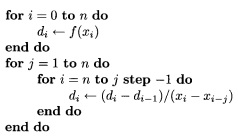
\includegraphics[scale=1.0]{Kincaid}
    \centering
    \caption{Pseudokod algorytmu zaimplementowanego w funkcji \textit{ilorazyRoznicowe}}
  \end{figure}
\chapter{Zadanie 2.}
  \section{Krótki opis problemu}
    Głownym celem tego zadania było zaimplementowanie funkcji \textit{warNewton}, która oblicza wartość wielomianu interpolacyjnego stopnia n w postaci Newtona $N_{n}(x)$ w punkcie $x=t$ za pomocą uogólnionego algorytmu Hornera \textbf{W czasie O(n)!}
  \section{Rozwiazanie}
    Rozwiązanie znajduje się w pliku \textit{header.jl}, w module \textit{Functions}. Korzystając z zadania 8 z listy nr 4 (ćwiczenia) autorstwa Profesora \textbf{Pawła Zielińskiego} skorzystamy z uogólnionych wzorów Hornera w celu zaimplementowania podanej funkcjonalności. W funkcji znajduje się tylko jedna pętla, wykonująca się maksymalnie tyle razy, jak długi jest wektor, na którym operuje, czyli $n+1$ razy, co daje nam złożoność obliczeniową $O(n)$ (zgodnie z poleceniem).
    \begin{figure}[H]
      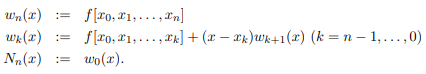
\includegraphics[scale=1.0]{warNewton}
      \centering
      \caption{Wzory wykorzystane w implementacji funkcji \textit{warNewton}}
    \end{figure}
\chapter{Zadanie 3.}
  \section{Krótki opis problemu}
    Głównym celem tego zadania było zaimplementowanie funkcji \textit{naturalna}, która oblicza współczynniki postaci naturalnej znając współczynniki wielomianu interpolacyjnego w Postaci Newtona oraz węzły (dane z oznaczeniami dokładnie opisane są w pliku \textit{header.jl}, w komentarzu dokumentującym funkcję) \textbf{W czasie $O(n^{2})$!}
  \section{Rozwiazanie}
    Rozwiązanie znajduje się w pliku \textit{header.jl}, w module \textit{Functions}. W wielomianie interpolującym, współczynnikiem stojącym przy najwyższej potędze ($x^{n}$) jest $c_{n}$. Korzystając z ów wiedzy możemy obliczyć kolejne współczynniki zaczynając od najwyższej potęgi i przy kolejnych iteracjach zmieniać współczynniki w taki sposób, aby były one w każdym momencie w postaciach naturalnych. W kolejnych iteracjach będziemy korzystać z obliczonych wcześniej współczynników postaci naturalnej do zaktualizowania ich o nowe potęgi. Z racji tego, że w funkcji znajdują się dwie zagnieżdżone pętle, która maksymalnie mogą wykonać się $n$ razy otrzymujemy złożoność na poziomie \textbf{O($n^{2}$)}.
\chapter{Zadanie 4.}
  \section{Krótki opis problemu}
    Głównym celem tego zadania było zaimplementowanie funkcji rysującej wielomian interpolacyjny i interpolowaną funkcję na zadanym przedziale $[a,b]$
  \section{Rozwiazanie}
    Rozwiązanie znajduje się w pliku \textit{header.jl}, w module \textit{Functions}. Dzielimy przedział na $n$ części i obliczamy wartości funkcji przekazanej jako argument dla wyznaczonych w wyniku podziału wartości $x$. Wyniki przechowujemy w specjalnych tablicach. Kolejnym krokiem jest wyznaczenie ilorazów różnicowych na podstawie otrzymanych wyników. Następnie dla otrzymania lepszego graficznego przedstawienia dzielimy przedział na $n*10$ części, gdzie 10 jest z góry ustaloną dodatkową gęstością- w ten sposób łatwiej nam będzie zauważyć zjawiska, które zachodzą w trakcie interpolacji wielomianem. Powtarzamy poprzednie czynności, ponownie otrzymane wyniki tablicujemy (oczywiście bez wyznaczenia kolejnych ilorazów różnicowych), a otrzymane tablice przedstawiamy graficznie przy pomocy funkcji \textit{plot} z pakietu \textit{PyPlot}
\chapter{Zadanie 5.}
  \section{Krótki opis problemu}
    Celem tego zadania było przetestowanie wcześniej zaimplementowanych funkcji na dwóch przykładach:
    \begin{enumerate}
      \item $e^{x}$ na przedziale $[0,1]$ dla $n=5,10,15$
      \item $x^{2}*sin(x)$ na przedziale $[-1,1]$ dla $n=5,10,15$
    \end{enumerate}
  \section{Rozwiazanie}
    Rozwiązanie znajduje się w pliku o nazwie \textit{zad5.jl}. Funkcje \textbf{a i b} implementują odpowiednio funkcje $e^{x}$ i $x^{2}*sin(x)$. Funkcja \textit{main()} odpowiada za rozruch programu.
  \section{Wyniki oraz ich interpretacje}
    Wykresy przedstawiające otrzymane rozwiązania:
    \begin{figure}[H]
      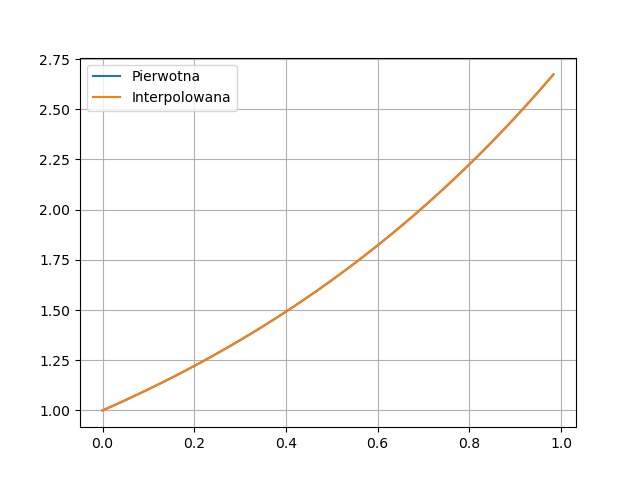
\includegraphics[scale=0.75]{a-5}
      \centering
      \caption{Wykres funkcji $e^{x}$ dla $n=5$}
    \end{figure}
    \begin{figure}[H]
      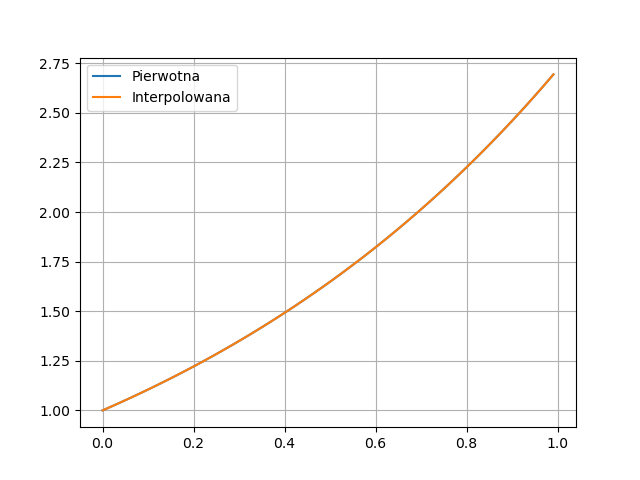
\includegraphics[scale=0.75]{a-10}
      \centering
      \caption{Wykres funkcji $e^{x}$ dla $n=10$}
    \end{figure}
    \begin{figure}[H]
      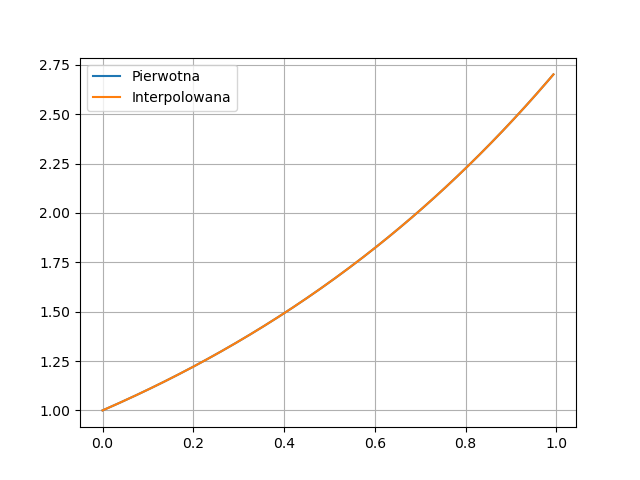
\includegraphics[scale=0.75]{a-15}
      \centering
      \caption{Wykres funkcji $e^{x}$ dla $n=15$}
    \end{figure}
    \begin{figure}[H]
      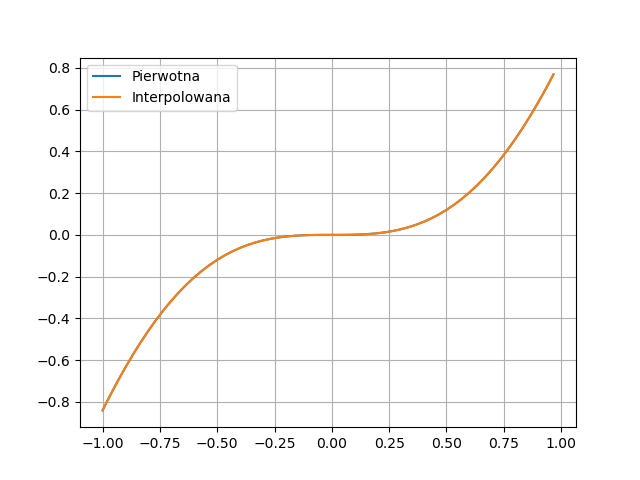
\includegraphics[scale=0.75]{b-5}
      \centering
      \caption{Wykres funkcji $x^{2}*sin(x)$ dla $n=5$}
    \end{figure}
    \begin{figure}[H]
      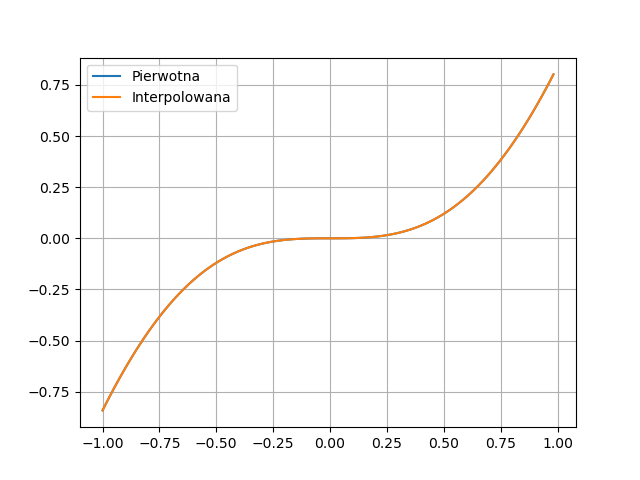
\includegraphics[scale=0.75]{b-10}
      \centering
      \caption{Wykres funkcji $x^{2}*sin(x)$ dla $n=10$}
    \end{figure}
    \begin{figure}[H]
      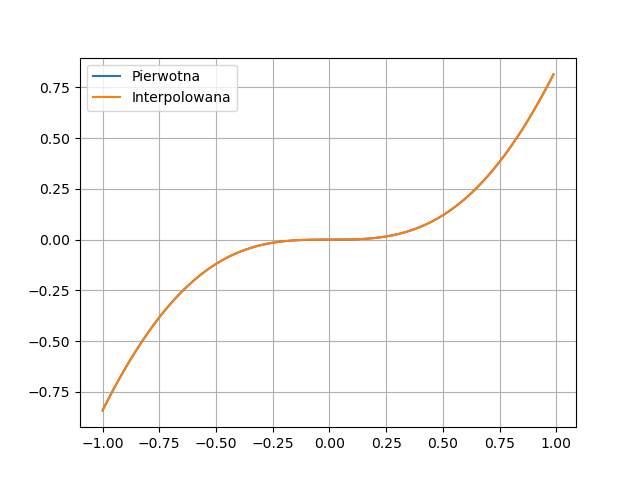
\includegraphics[scale=0.75]{b-15}
      \centering
      \caption{Wykres funkcji $x^{2}*sin(x)$ dla $n=15$}
    \end{figure}
    \textbf{Interpretacja: } Zauważamy, iż dana funkcja oraz jej interpolacja wielomianem są wręcz tożsame. Wynika to z faktu, iż ów funkcje mają stałą pochodną oraz niewiele różnią się między kolejnymi sprawdzanymi argumentami
  \section{Wnioski}
    Ze względu na stały znak pochodnej oraz niewielkie różnice w wartościach zwracanych przez funkcję, wielomian interpolacyjnych bardzo dokładnie interpoluje podane funkcje w podanych zakresach.

\chapter{Zadanie 6.}
  \section{Krótki opis problemu}
    Celem tego zadania było przetestowanie wcześniej zaimplementowanych funkcji na dwóch przykładach:
    \begin{enumerate}
      \item $|x|$ na przedziale $[-1,1]$ dla $n=5,10,15$
      \item $\frac{1}{1+x^{2}}$ na przedziale $[-5,5]$ dla $n=5,10,15$
    \end{enumerate}
  \section{Rozwiazanie}
    Rozwiązanie znajduje się w pliku o nazwie \textit{zad6.jl}. Funkcje \textbf{c i d} implementują odpowiednio funkcje $|x|$ i $\frac{1}{1+x^{2}}$. Funkcja \textit{main()} odpowiada za rozruch programu.
  \section{Wyniki oraz ich interpretacje}
    Wykresy przedstawiające otrzymane rozwiązania:
    \begin{figure}[H]
      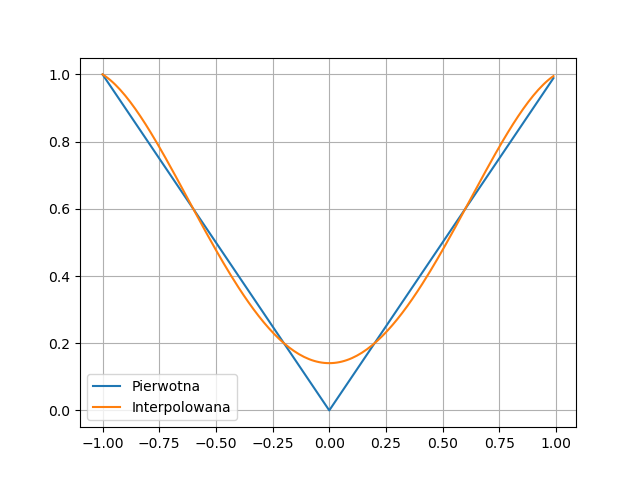
\includegraphics[scale=0.75]{c-5}
      \centering
      \caption{Wykres funkcji $|x|$ dla $n=5$}
    \end{figure}
    \begin{figure}[H]
      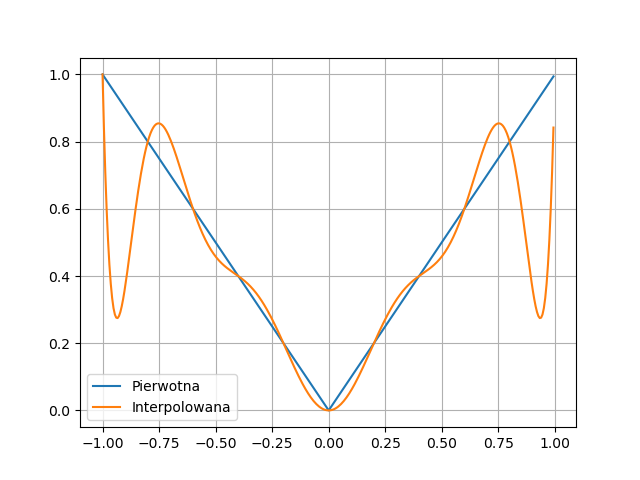
\includegraphics[scale=0.75]{c-10}
      \centering
      \caption{Wykres funkcji $|x|$ dla $n=10$}
    \end{figure}
    \begin{figure}[H]
      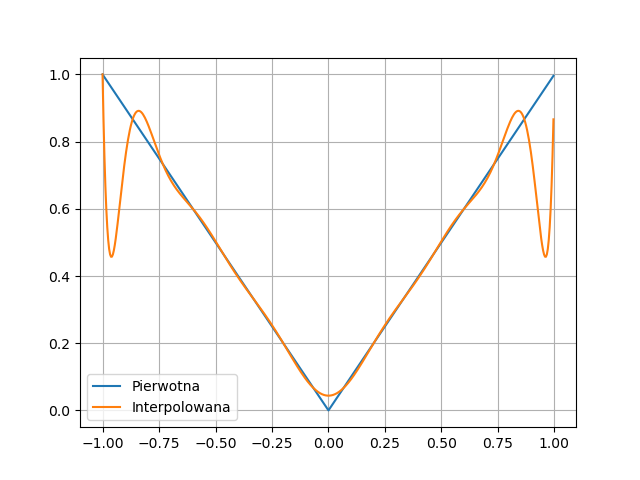
\includegraphics[scale=0.75]{c-15}
      \centering
      \caption{Wykres funkcji $|x|$dla $n=15$}
    \end{figure}
    \begin{figure}[H]
      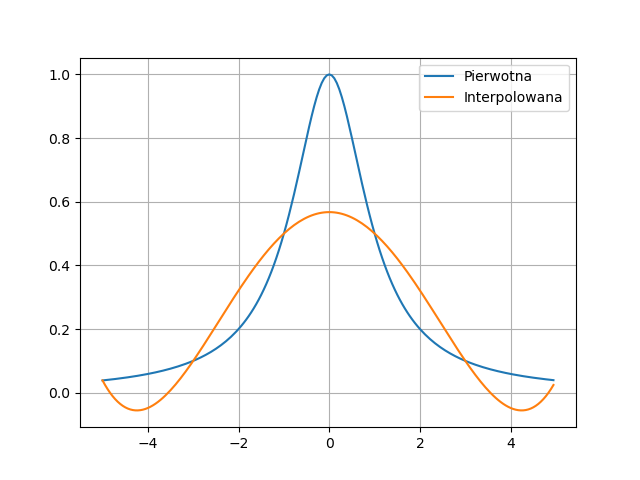
\includegraphics[scale=0.75]{d-5}
      \centering
      \caption{Wykres funkcji $\frac{1}{1+x^{2}}$ dla $n=5$}
    \end{figure}
    \begin{figure}[H]
      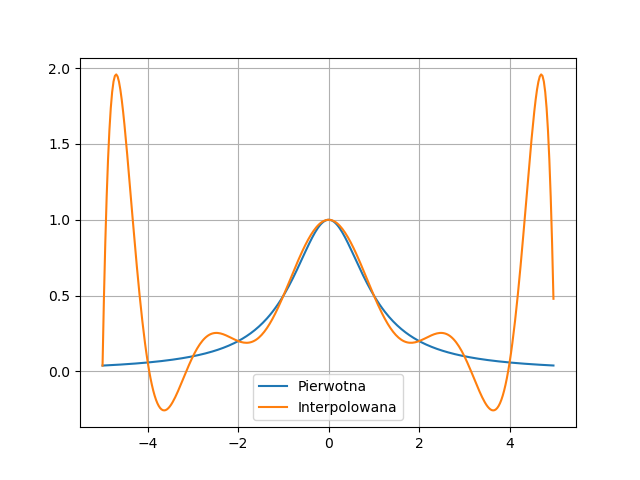
\includegraphics[scale=0.75]{d-10}
      \centering
      \caption{Wykres funkcji $\frac{1}{1+x^{2}}$ dla $n=10$}
    \end{figure}
    \begin{figure}[H]
      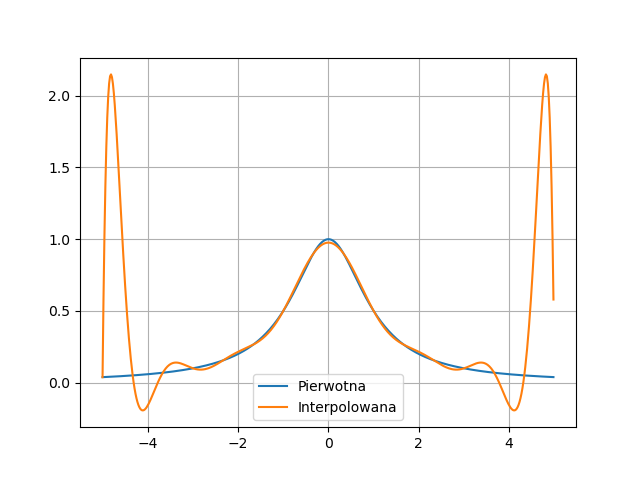
\includegraphics[scale=0.75]{d-15}
      \centering
      \caption{Wykres funkcji $\frac{1}{1+x^{2}}$ dla $n=15$}
    \end{figure}
    \textbf{Interpretacja: } Zauważamy, iż w odróżnieniu od poprzedniego przypadku wykres funkcji jak i jej interpolacja wielomianem zdecydowanie się różnią. To co jest charakterystyczne to fakt, iż im mniejsze n tym mniejsza  dokładność w środkowej partii przedziału, a większą na jej krańcach, co dynamicznie zmienia się ze wzrostem n (już dla 10, czy 15 widzimy większą dokładność w środku, aniżeli na krańcach przedziału, gdzie funkcja zdecydowanie odbiega od pierwowzoru). Zauważamy duże odchylenia w miejscach, w których pochodna zmienia znak oraz wartości funkcji między kolejnymi węzłami są odpowiednio duże.
  \section{Wnioski}
    Zauważamy, iż ze wzrostem stopnia wielomianu interpolacyjnego zyskujemy dokładność w środkowych partiach przedziału na rzecz dokładności na jej krańcach. Wynika to ze swego rodzaju paradoksu opisanego przez niemieckiego matematyka \textbf{Carla Rungego}, który zauważył, iż zachodzi pogorszenie jakości interpolacji wielomianowej, mimo zwiększenia liczby jej węzłów. Dodatkowo stwierdził, iż wielomiany wysokich stopniów nie nadają się do interpolacji, gdy w interpolacji korzystamy z węzłów równoodległych. Aby uniknąć tego efektu stosuje się interpolacje z węzłami gęściej upakowanymi na krancach przedziałów. (Jednym z rozwiązań jest interpolacja, której węzły są miejscami zerowymi wielomianu Czebyszewa n-tego stopnia).  
\end{document}